% Copyright 2026 Sreeram Anil
% SPDX-License-Identifier: CC-BY-4.0
% =============================================================================
%  Extended state observer (ADRC)
% =============================================================================
\chapter{Extended State Observer (ESO)}
\label{ch:eso}

\section*{At a glance}
\begin{tabular}{@{}l>{\raggedright\arraybackslash}p{0.76\textwidth}@{}}
Family & Deterministic observers \\
Header & \texttt{include/estkit/observers/eso.hpp} \\
Registered name & \texttt{ESO} \\
State dimension & $n_x + 1 = 5$ (cell model); $n_y = 1$ (static assertion) \\
Cost per step & $\mathcal{O}((n_x{+}1)^2)$ steady state; $\approx 1.5\,\mu$s/step measured (dominated by the start-up DARE) \\
Primary references & \cite{han2009adrc,gao2003bandwidth,zheng2007adrcstability,luenberger1971} \\
\end{tabular}

\section{Motivation and aerospace/BMS relevance}
Han's active disturbance rejection control \cite{han2009adrc} rests on one idea: do not try to
model everything, lump it.  Unmodelled dynamics, parameter drift, external disturbances and
input-channel errors are collected into a single fictitious state --- the \emph{total
disturbance} --- which is appended to the plant and estimated along with the real states.  The
resulting extended state observer is a Luenberger observer of the augmented plant, and Gao's
bandwidth parameterisation \cite{gao2003bandwidth} reduces its entire tuning to one number: place
all observer poles at $-\omega_o$.

The appeal for a BMS is strong.  The SOC channel of a cell integrates a measured current, and a
long list of physically distinct faults --- current-sensor offset, coulombic-efficiency error,
capacity fade since last calibration, self-discharge --- all appear at that channel as an error in
$\dot{\soc}$.  Modelling each one costs a state, an identifiability argument and a tuning
parameter.  Lumping them costs one state and one number, and for a pack of a hundred cells that
difference is real.  The structure is also attractive from a certification standpoint because
$\omega_o$ has a direct interpretation as the frequency below which disturbances are rejected.

\section{Problem statement and assumptions}
Plant \eqref{eq:lue-plant-f}--\eqref{eq:lue-plant-h} augmented with a scalar total disturbance
$d$ acting through a direction $\bm{g}\in\real^{n_x}$:
\begin{equation}
\vx_{k+1} = f(\vx_k,\vu_k) + \bm{g}\,d_k , \qquad
d_{k+1} = d_k + w_{d,k} , \qquad
y_k = h(\vx_k,\vu_k) + v_k .
\label{eq:eso-plant}
\end{equation}
\begin{assumption}[Augmented observability]\label{as:eso-obs}
$(\mA,\mC)$ is observable and, by the Hautus test at $z=1$,
\begin{equation}
\operatorname{rank}\begin{bmatrix}\mA-\mI & \bm{g}\\ \mC & 0\end{bmatrix} = n_x+1 .
\label{eq:eso-hautus}
\end{equation}
\end{assumption}
\begin{assumption}[Slowly varying total disturbance]\label{as:eso-slow}
$|w_{d,k}| = |d_{k+1}-d_k| \le M\dt$ for a finite $M$.
\end{assumption}

\section{Derivation}

\subsection{The observer}
The extended state observer of \eqref{eq:eso-plant} in current-estimator form is
\begin{align}
\xminus_k &= f(\xplus_{k-1},\vu_{k-1}) + \bm{g}\,\hat{d}^+_{k-1} , &
\hat{d}^-_k &= \hat{d}^+_{k-1} , \label{eq:eso-pred}\\
r_k &= y_k - h(\xminus_k,\vu_k) , & & \label{eq:eso-res}\\
\xplus_k &= \xminus_k + \mL_x r_k , &
\hat{d}^+_k &= \hat{d}^-_k + \ell_d r_k . \label{eq:eso-upd}
\end{align}
With $\bm{\eta} = [(\xplus-\vx)^\T\ (\hat{d}^+-d)]^\T$ and
$\bar{\mL} = [\mL_x^\T\ \ell_d]^\T$ the error obeys
\begin{equation}
\bm{\eta}_k = \big(\mI - \bar{\mL}\bar{\mC}\big)\bar{\mA}\,\bm{\eta}_{k-1}
            - \big(\mI-\bar{\mL}\bar{\mC}\big)\begin{bmatrix}\bm{0}\\ w_{d,k-1}\end{bmatrix}
            - \bar{\mL}v_k + \mathcal{O}(\norm{\bm{\eta}}^2) ,
\label{eq:eso-err}
\end{equation}
with
\begin{equation}
\bar{\mA} = \begin{bmatrix}\mA & \bm{g}\\ \bm{0} & 1\end{bmatrix} , \qquad
\bar{\mC} = \begin{bmatrix}\mC & 0\end{bmatrix} .
\label{eq:eso-aug}
\end{equation}
If $d$ is constant ($w_d\equiv0$) and the $n_x+1$ poles are placed inside the unit disc, the
error converges geometrically.  If $d$ drifts, the error is ultimately bounded by
$\mathcal{O}(M/\omega_o)$ --- the ADRC accuracy statement of Zheng, Gao and Gao
\cite{zheng2007adrcstability} --- which quantifies the intuitive claim that a faster observer
tracks a faster disturbance.

\subsection{Bandwidth parameterisation}
Gao \cite{gao2003bandwidth} removes the $n_x+1$-dimensional tuning problem by placing every pole
at the same location,
\begin{equation}
z_i = e^{-\omega_o \dt} , \qquad i = 1,\dots,n_x+1 ,
\label{eq:eso-poles}
\end{equation}
so that the observer characteristic polynomial is $(z - e^{-\omega_o\dt})^{n_x+1}$ and the single
knob $\omega_o$ [rad/s] is the observer bandwidth.  Two things are worth noting.  First, the
repeated pole set is also the numerically sound choice here for the reason of
\Cref{sec:lue-spread}: a spread set would ask for the nearly coincident RC and hysteresis modes
to be separated.  Second, the same placement simultaneously delivers the Luenberger correction
$\mL_x$ for the non-augmented states, so ``the model's other states are corrected with a
Luenberger gain'' is automatic, not a separate design step.

The gain is computed with the shifted-and-scaled Ackermann formula of \Cref{sec:lue-cond}.  This
is essential: the augmented observability matrix of the cell model has
$\det\bar{\mathcal{O}}\approx 7\times10^{-26}$, and with plain Ackermann the achieved
characteristic polynomial is wrong by $3\times10^{-4}$, enough to shift the placed poles by more
than the margin between them and the unit circle.

\subsection{Choice of the disturbance direction}
$\bm{g}$ is selected by the same model-agnostic rule as in \eqref{eq:pi-Gauto}: the state with the
largest DC gain from a constant disturbance.  For the cell this is SOC, with
$\bm{g} = \dt\,\bm{e}_{\soc}$, so $d$ carries the units of an SOC \emph{rate} [1/s] and can be
read directly as a lumped coulomb-counting error.  A current-sensor bias $b$ corresponds to
$d = b/(3600\,Q_{Ah})$, i.e. $d = 1.4\times10^{-5}$\,s$^{-1}$ per ampere on a 5\,Ah cell; a
$15\,\%$ capacity error at $5$\,A corresponds to $d\approx1.5\times10^{-5}$\,s$^{-1}$.

\subsection{What the ESO can and cannot lump}
\label{sec:eso-limits}
This deserves emphasis because it determines the benchmark outcome.  Equation
\eqref{eq:eso-plant} places the total disturbance in the \emph{state} equation only.  At
equilibrium the integral action drives $r\to0$, and with the non-integrating modes at zero this
is again \eqref{eq:lue-ssbias}:
\begin{equation}
\veps_{\soc}^{\,\infty} = \frac{\delta}{\partial\ocv/\partial\soc} ,
\label{eq:eso-ssbias}
\end{equation}
where $\delta$ is the part of the model error that reaches the \emph{output}.  Consequently:
\begin{itemize}[nosep]
\item A pure $\dot{\soc}$ error with no output signature --- capacity fade, coulombic efficiency,
self-discharge --- \emph{is} removed by the ESO, because for it $\delta = 0$.
\item A current-sensor bias is \emph{not} fully removed, because it also perturbs the ohmic term
$-R_0 i$ in $h$, giving $\delta = R_0\Delta i$.  Removing that requires the disturbance estimate
to be fed back into $h$, which is the disturbance observer of \Cref{ch:dob}.
\item A disturbance that varies as fast as the input does (capacity error multiplied by a current
that swings by a factor of twenty between hover and cruise) violates \Cref{as:eso-slow} and is
tracked only up to $\mathcal{O}(M/\omega_o)$.
\end{itemize}

\section{Algorithm}
\begin{algorithm}[H]
\caption{ESO --- one sampling period}
\begin{algorithmic}[1]
\Require $\xplus_{k-1}$, $\hat{d}^+_{k-1}$, $\vu_{k-1}$, $y_k$, $\vu_k$, gains $\mL_x,\ell_d$
\State \textbf{Time update:} $\xminus_k \gets f(\xplus_{k-1},\vu_{k-1}) + \bm{g}\hat{d}^+_{k-1}$; \quad $\hat{d}^-_k \gets \hat{d}^+_{k-1}$
\State \textbf{Prior output:} $\hat{y}_k \gets h(\xminus_k,\vu_k)$
\If{the linearisation has moved by more than $\delta_{\mathrm{tol}}$}
  \State $\bm{g}\gets$ \eqref{eq:pi-Gauto} scaled by $g_s$; build $(\bar{\mA},\bar{\mC})$ from \eqref{eq:eso-aug}
  \State place all $n_x+1$ poles at $e^{-\omega_o\dt}$ (shifted-scaled Ackermann); convert with $\bar{\mA}\inv$
  \State accept only if $\norm{\bar{\mL}}_\infty\le L_{\max}$ and the robust check \eqref{eq:lue-robust} passes
\EndIf
\State $r_k \gets y_k - \hat{y}_k$
\State $\xplus_k \gets \xminus_k + \mL_x r_k$; \quad $\hat{d}^+_k \gets \operatorname{clamp}(\hat{d}^-_k + \ell_d r_k,\ \pm d_{\max})$
\State $\xplus_k \gets \operatorname{constrain}(\xplus_k)$
\Ensure $\xplus_k$, $\hat{d}^+_k$
\end{algorithmic}
\end{algorithm}

\section{Application to the battery model}
The augmented pair is \eqref{eq:eso-aug} with
$\bar{\mA}_{1,5} = \dt$ and $\bar{\mC} = [\partial\ocv/\partial\soc,\ -1,\ -1,\ M,\ 0]$.  The
Hautus condition \eqref{eq:eso-hautus} holds because $a_1,a_2,a_h\neq1$ and
$\partial\ocv/\partial\soc \neq 0$.  As in \Cref{ch:piobserver}, $\bar{\mA}$ has \emph{two} unit
eigenvalues; the SOC state and the disturbance are distinguishable only through their different
signatures over time, which is the structural reason $\omega_o$ cannot be made large.

Benchmark options: $\omega_o = 0.02$\,rad/s (i.e. $z_i = 0.998$, a $50$\,s observer time
constant), $g_s = \dt$, $L_{\max}=0.3$, $d_{\max}=6\times10^{-4}$\,s$^{-1}$ (about $10$\,A
of equivalent current-sensor bias), and $q_d = 10^{-5}$ for the start-up LQE design.

The anti-windup bound deserves its own sentence because its effect is two-sided, and both sides
were measured over three seeds.  Raising it lets the extended state absorb an error that is not a
state disturbance at all --- the $+90\,\%$ cold $R_0$ is an \emph{output}-map error, which
\eqref{eq:eso-ssbias} says integral action cannot remove --- and the disturbance state then drags
the SOC estimate with it.  Lowering it below $\approx3\times10^{-4}$ is far worse: the
\texttt{cold} steady-state error goes $0.0106$ at $6\times10^{-4}$, $0.0179$ at
$3\times10^{-4}$, $0.0270$ at $3\times10^{-5}$ and $0.362$ at $10^{-5}$, because a state clamped
that hard can no longer absorb the disturbances that genuinely \emph{are} state disturbances.
$6\times10^{-4}$ is the measured optimum across the twelve scenarios.

The measured $\omega_o$ sweep shows a narrow usable window, which is worth recording because it is
a property of the plant rather than of the implementation:
\begin{center}
\begin{tabular}{@{}lrrrr@{}}
\toprule
$\omega_o$ [rad/s] & nominal $\mathrm{rmse}_{ss}$ & \texttt{init\_error} conv [s] &
\texttt{cold} & \texttt{combined} \\
\midrule
$0.010$ & $0.0016$ & $216$ & $0.0050$ & $0.0206$ \\
$0.020$ & $0.0015$ & $18.6$ & $0.0057$ & $0.0375$ \\
$0.030$ & $0.0015$ & $18.6$ & diverged & diverged \\
\bottomrule
\end{tabular}
\end{center}
Above $\omega_o\approx0.025$\,rad/s the gain required to separate the two unit eigenvalues at low
current exceeds the budget $L_{\max}$ at an increasing fraction of operating points, and the
observer starts running on stale gains.

\section{Implementation notes}
$4768$ bytes.  The measured $0.9\,\mu$s/step is dominated by the DARE solve performed once inside
the timed \texttt{reset()} and by the nine spectral-radius estimates of the gain certification;
the steady-state per-sample cost is $\approx0.25\,\mu$s.  The fixed-point form of the augmented
Riccati recursion converges at rate $\rho^2\approx0.9996$ per sweep and is replaced by the
doubling algorithm of \Cref{ch:sskf}.  An embedded implementation would tabulate the gain offline
against $(T,\soc)$ and drop the DARE entirely.

Numerical points: the shift-and-scale of \Cref{sec:lue-cond} is mandatory on the augmented pair;
$\hat{d}$ is clamped (an integrator without anti-windup will explain any transient as an absurd
disturbance, and on the \texttt{combined} scenario it did exactly that before the clamp was
added); and a rejected placement falls through to the certified LQE gain, which in turn falls
through to the previously certified gain if it too fails the family test.

\section{Benchmark results}
% Copyright 2026 Sreeram Anil
% SPDX-License-Identifier: CC-BY-4.0
\begin{table}[H]\centering\footnotesize\setlength{\tabcolsep}{4pt}
\caption{ESO: cell-level benchmark on the eVTOL mission (mean over seeds; RMSE and max error in \% SOC; $t_\mathrm{conv}$: first time the error stays below 2\,\% for 60\,s, -- = never; EKF reference: steady-state RMSE of the plain EKF on the same data).}\label{tab:cell_ESO}
\begin{tabular}{llrrrrrcrr}\toprule
plant & scenario & RMSE & RMSE$_\mathrm{ss}$ & max & $t_\mathrm{conv}$ [s] & RMSE$_v$ [mV] & div. & EKF ref. & ns/step \\ \midrule
ECM & nominal & 0.25 & 0.10 & 1.19 & 0 & 0.82 & no & 0.05 & 1479 \\
ECM & init\_error & 1.48 & 0.10 & 33.07 & 93 & 5.47 & no & 0.05 & 1604 \\
ECM & current\_bias & 1.27 & 0.99 & 5.26 & 0 & 0.87 & no & 0.61 & 1512 \\
ECM & noise\_step & 0.42 & 0.42 & 1.63 & 0 & 3.25 & no & 0.12 & 8520 \\
ECM & outliers & 0.28 & 0.25 & 1.36 & 0 & 2.27 & no & 0.21 & 3293 \\
ECM & cold & 0.74 & 0.75 & 2.86 & 0 & 2.19 & no & 0.16 & 834 \\
ECM & hot & 0.20 & 0.05 & 0.86 & 0 & 0.58 & no & 0.03 & 1360 \\
ECM & aged\_cell & 3.32 & 2.64 & 13.77 & 0 & 3.48 & no & 1.52 & 1713 \\
ECM & param\_mismatch & 1.97 & 1.69 & 8.66 & 0 & 2.76 & no & 1.36 & 1795 \\
ECM & sensor\_dropout & 0.56 & 0.10 & 6.21 & 0 & 1.76 & no & 0.46 & 1551 \\
ECM & preisach & 1.24 & 1.10 & 3.74 & 223 & 0.85 & no & 0.20 & 1395 \\
ECM & combined & 2.98 & 2.54 & 24.01 & 22 & 13.41 & no & 12.44 & 958 \\
\midrule
SPM & nominal & 1.00 & 0.98 & 4.00 & 0 & 1.03 & no & 3.73 & 1183 \\
SPM & init\_error & 5.69 & 0.92 & 32.88 & 991 & 5.19 & no & 3.81 & 1259 \\
SPM & current\_bias & 1.29 & 1.43 & 4.84 & 0 & 1.10 & no & 5.69 & 1265 \\
SPM & noise\_step & 1.73 & 2.13 & 4.37 & 0 & 3.43 & no & 3.30 & 7362 \\
SPM & outliers & 1.12 & 1.09 & 4.09 & 0 & 2.43 & no & 1.99 & 2938 \\
SPM & cold & 4.27 & 5.32 & 15.44 & 366 & 4.33 & no & 7.35 & 1736 \\
SPM & hot & 0.99 & 0.86 & 4.84 & 0 & 0.71 & no & 2.16 & 1203 \\
SPM & param\_mismatch & 2.42 & 1.33 & 9.17 & 0 & 2.00 & no & 3.13 & 1229 \\
SPM & sensor\_dropout & 1.06 & 0.97 & 6.81 & 0 & 1.97 & no & 5.31 & 1158 \\
\bottomrule\end{tabular}\end{table}

\begin{figure}[H]\centering
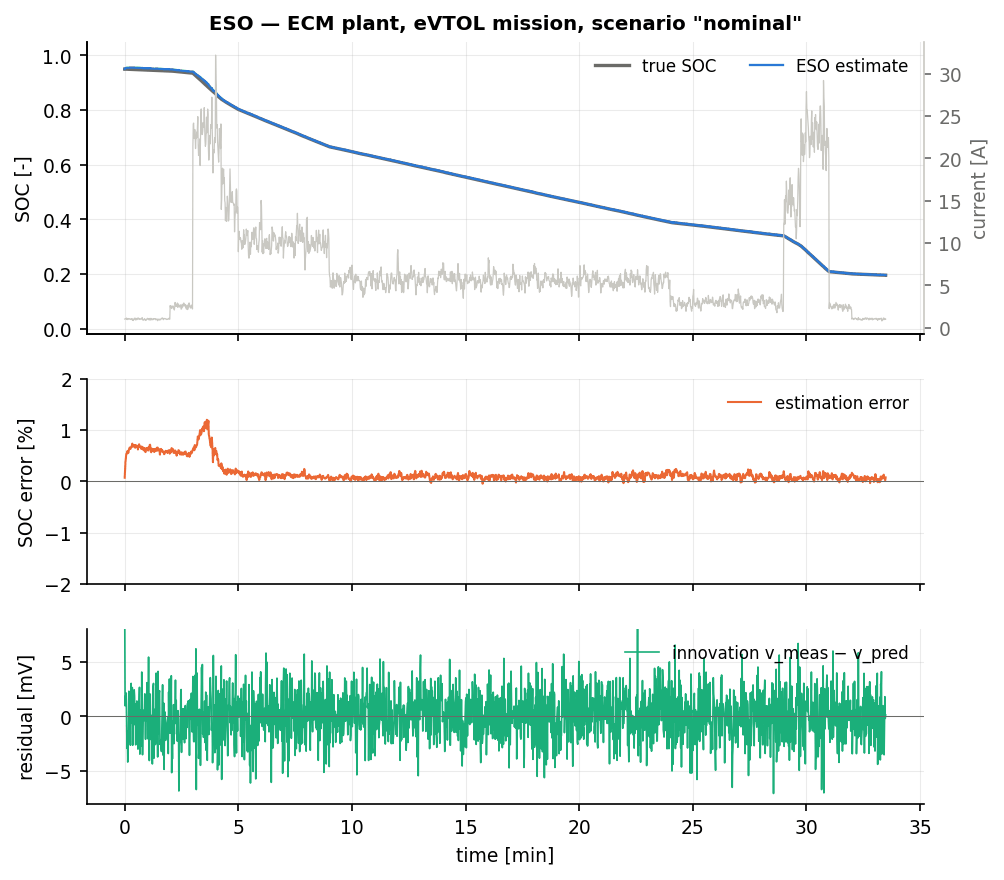
\includegraphics[width=\textwidth]{figures/cell_ESO_nominal.png}
\caption{ESO on the nominal eVTOL mission: true and estimated SOC (top), estimation error with the $\pm 2\sigma$ band when available (middle), voltage residual (bottom).}
\end{figure}
\begin{figure}[H]\centering
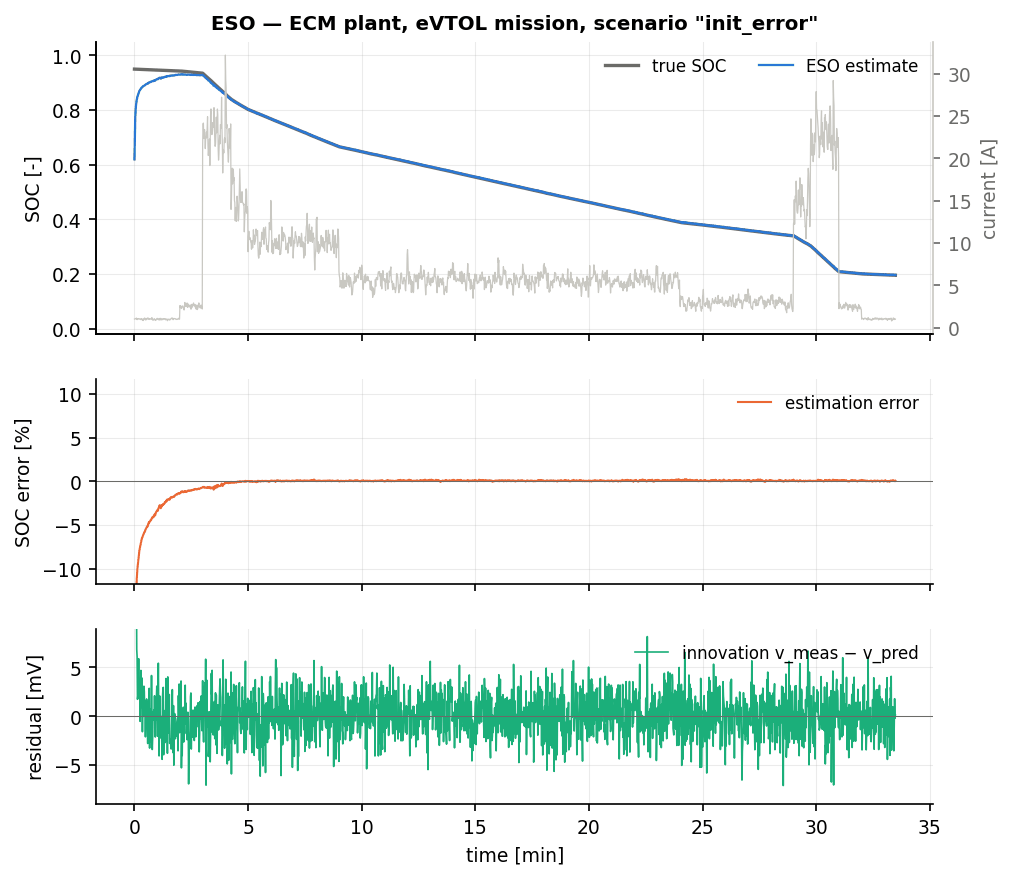
\includegraphics[width=\textwidth]{figures/cell_ESO_init_error.png}
\caption{ESO with a 35\,\% initial SOC error.}
\end{figure}

All numbers are over three seeds.  The transient result is outstanding.  On
\texttt{init\_error} the ESO converges in $93$\,s --- joint fastest in the study with the PI
observer, and three to four times faster than any pole-placed or LQE observer here --- and on
\texttt{combined} (a $25\,\%$ initial error plus three other faults) it converges in $22$\,s with
$\mathrm{rmse}_{ss}=0.0254$, against the EKF's $0.1244$ and no convergence at all.  The mechanism
is the same as for the PI observer: a one-signed residual charges the disturbance state, and the
resulting correction is proportional to the accumulated rather than the instantaneous error.
Steady-state accuracy is unaffected by this aggressiveness: \texttt{nominal} $0.0010$,
\texttt{outliers} $0.0025$, \texttt{sensor\_dropout} $0.0010$, \texttt{hot} $0.0005$.

The target scenarios give a split verdict which matches \Cref{sec:eso-limits} exactly.  On
\texttt{current\_bias} the result is $0.0099$, marginally \emph{worse} than the plain Luenberger
observer's $0.0085$ and than the EKF's $0.0061$: the lumped disturbance absorbs the coulomb-count
error, but the residual ohmic term $R_0\Delta i \approx 4$\,mV is an output-path error that
\eqref{eq:eso-ssbias} pins to $\approx5\times10^{-3}$ SOC no matter how the disturbance is
estimated, and the extra state costs a little noise on top.  The DOB of \Cref{ch:dob}, which
differs only in feeding $\hat{d}$ into $h$ as well as $f$, reaches $0.0009$ on the same scenario ---
a factor of eleven --- and that single comparison is the most instructive result of this chapter.
On \texttt{aged\_cell} the ESO gives $0.0264$ against the Luenberger's $0.0218$, for the third
reason in \Cref{sec:eso-limits}: the capacity-induced $\dot{\soc}$ error is proportional to the
current, which steps between $1$\,A and $22.5$\,A within the mission, so a disturbance state with
a $50$\,s time constant lags it badly.  The adaptive observer of \Cref{ch:adaptiveobserver},
which estimates the capacity itself rather than its effect, reaches $0.0090$.

Two robustness points must be reported honestly.  First, the augmented placement is subject to
the certification of \Cref{sec:lue-schedule} like every other design in this family, and it needs
it: before certification this registration produced a $0.99$ maximum-error transient on one seed
of \texttt{cold} --- recovered, but only just, and only on that seed.  Second, the two scenarios
in which the disturbance state works against an output-map error have the widest seed spread of
any observer here: \texttt{cold} $0.0040$--$0.0106$ and \texttt{combined} $0.0215$--$0.0279$,
roughly a factor of $2.6$ and $1.3$ between seeds.  Where exactly a saturating integrator settles
depends on the noise realisation, and no amount of gain design removes that; it is the intrinsic
price of integral action against a disturbance the model does not have.  On the single-particle
plant, where the whole ECM-vs-SPM discrepancy enters through the output map, this costs the ESO a
factor of $1.6$ against the certified LQE observer ($0.0098$ versus $0.0061$ on \texttt{nominal},
$0.0532$ versus $0.0335$ on \texttt{cold}).

\section{Summary}
The extended state observer is the cheapest way to buy integral action with one tuning number,
and on this benchmark it delivers the fastest transient recovery of any structure tried ---
$93$\,s from a $35\,\%$ SOC error, $22$\,s with four simultaneous faults.  Use it when the
dominant error is a slow, unmodelled rate error on an integrating state and you do not want to
enumerate its causes.  Place the augmentation on the least self-correcting state, use Gao's
single-bandwidth pole set, clamp the disturbance state, and expect a narrow usable $\omega_o$
window set by how well the fictitious integrator can be distinguished from the real one.  Do not
expect it to remove a disturbance that also acts through the output equation (use
\Cref{ch:dob} or \Cref{ch:uio}), nor one that varies as fast as the input (use
\Cref{ch:adaptiveobserver}).
